% chapter 6 
\chapter{游戏}

\section{GOG}
\begin{itemize}
\item 安装 lgogdownloader:

由于 GOG 平台没有 Linux 客户端,所以只能通过 命令行来下载。

\begin{lstlisting}
$ sudo apt install -y lgogdownloader

# 登陆 Gog 账号
$ sudo lgogdownloader --login 

# 查看自已的游戏库
$ sudo lgogdownloader --list

# 下载游戏,下载完成后,运行脚本即可。
$ sudo lgogdownloader --download --platform 4 --game <游戏名称>
\end{lstlisting}
\newpage

\section{steam}

与 gog 平台相比 steam 有自己的 Linux 客户端,并且速度游戏下载速度更快。

\item 下载客户端

下载 \href{https://store.steampowered.com/about/}{steam Linux 客户端} 

\begin{figure}[htp]  
	\centering
	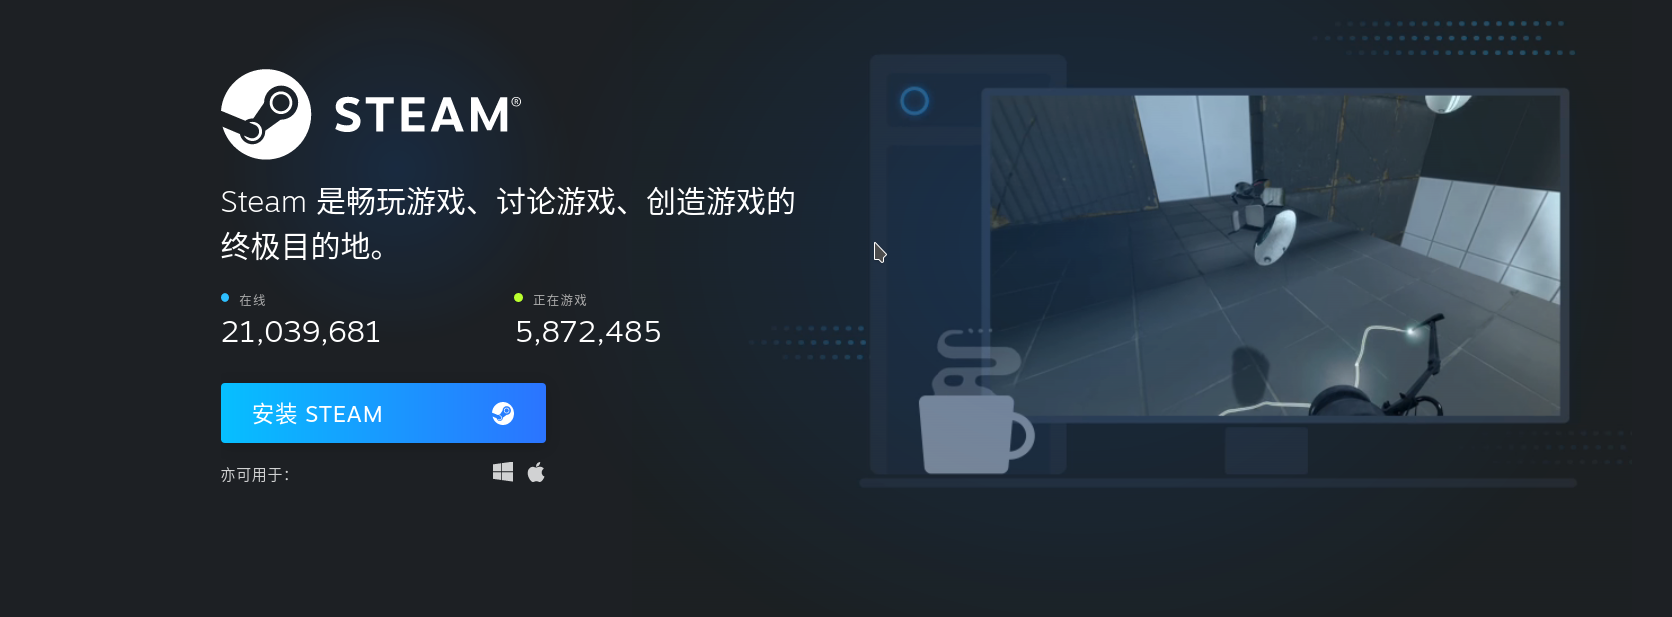
\includegraphics[width=0.8\textwidth]{./img/game/steam.png}
	\caption{下载页面} %caption是图片的标题
	\label{fig:steam} %此处的label相当于一个图片的专属标志,目的是方便上下文的引用
\end{figure}

\item 安装
\begin{lstlisting}
$ sudo dpkg -i steam_latest.deb
\end{lstlisting}

\end{itemize}
